\section{Regression}

\subsection{Bivariate Numerical Data Descriptive Methods}
\begin{objectives}
    \item Know how to draw graph for bivariate data
    \item Understand linear regression
    \item Know how to do regression for bivariate data
\end{objectives}
\vbox{}
\Index{Bivariate Data} is the set of numerical data from two measurements of a sample. These two measurements may have some kind of correlation and we need to represent this correlation using graphical method and linear regression.\\
\begin{examplebox}{Bivariate}
    We want to know the if there is a cause-effect relationship between students' AP stats score and time spent on practice problems, then we measure individual in the sample for score and practice time. The data has two variables in pairs.
\end{examplebox}
\begin{Center}
    \textbf{Graphical method}
\end{Center}
We use \textcolor{red}{Scatter-plot}. y is the \textcolor{blue}{Response Variable}, x is the \textcolor{blue}{Experimental Variable}. We draw them in one graph intending to find the \textcolor{red}{Cause-effect relation} between the two factors. In this scatter-plot, it's acceptable to have two y for the same x.
\begin{figure}[H]
    \centering
        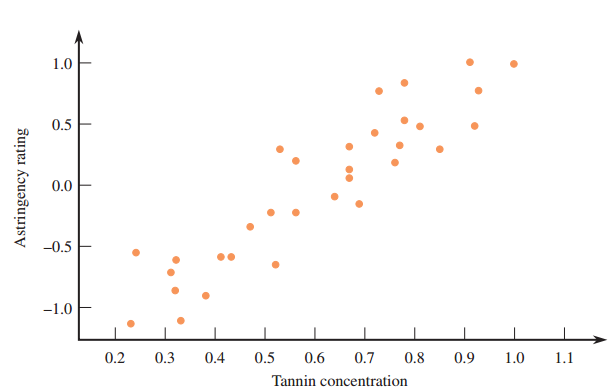
\includegraphics[width=100mm]{relation.png}
        \caption{Scatter-plot}
        \label{fig:my_label}
\end{figure}
From the example of representing bi-variate data using a scatter-plot above, we are able to see the pattern and relationship between x and y very clearly. In this example, it's clear that the response variable is positively related to the explanatory variable x. The relationship is roughly linear.
\vspace{6ex}
\begin{Center}
    \textbf{Regression}
\end{Center}
It's easy to observe that in the above scatter-plot there is a linear relation between x and y. And doing regression is we try to find a \textcolor{red}{linear function that can best represent the cause-and-effect relationship} between two features of one sample. We can do the regression using calculator.

\begin{equation}
    \hat{y}=b_0+b_1x_i
\end{equation}
Where \(\hat{y}\) is the \Index{y predicted}, \(b_0 b_1\) are two constants.\\
\begin{paragraph}{Residual}
    Though we try to find the best, there is difference between the predicted value and the actual value. This difference is called as the \Index{Residual}: The error due to regression, also the unexplained deviation.
\end{paragraph}
\begin{equation}
    e_i=y_i-\hat{y}_i
\end{equation}
The linear function we are looking for is the one that minimizes the \Index{Sum of Square Residuals/SSR}. This method of doing regression is \Index{Least Square Regression}.
\begin{equation}
    \sum{{e_i}^2}=\sum{(y_i-\hat{y}_i)^2}
\end{equation}
\Index{Time Series}: When we have repeated measurements for several times, we can think of it as Bivariate data, where the x-axis is time. The points on the time-series though have to be connected starting from the origin. In a time-series, we can find \textcolor{red}{trend} of the variable we are considering.
\begin{figure}[H]
    \centering
        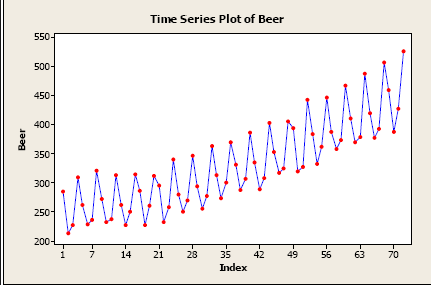
\includegraphics[width=100mm]{times.png}
        \caption{Time series}
        \label{fig:my_label}
\end{figure}

\subsection{More about Regression}
\begin{objectives}
    \item Understand coefficients in a regression
    \item Know variability of a regression    
\end{objectives}
\vbox{}
With a bunch of data of x and y, how do we calculate the two important constants in the linear regression \(\hat{y}=b_0+b_1x_i\)?
 \vspace{6ex}
\begin{Center}
    \textbf{Variance and Covariance}
\end{Center}
    First, we need to calculate the \textcolor{red}{variance} and \textcolor{red}{Covariance} of all x and y data.
    \begin{equation}
        Var(x)=\frac{\sum{(x_i-\bar{x})(x_i-\bar{x})}}{n}    
    \end{equation}
    \begin{equation}
        Var(y)=\frac{\sum{(y_i-\bar{y})(y_i-\bar{y})}}{n}
    \end{equation}
    \begin{equation}
        Covar(x,y)=\frac{\sum{(x_i-\bar{x})(y_i-\bar{y})}}{n}
    \end{equation}
\begin{itemize}
    \item \Index{Variance}: The measure of the average deviation form the mean.
    \item \Index{Covariance}: The measure of how much of the variability in the response variable(y) can be explained by the variability in the explanatory variability(x).
\end{itemize}
And based on the above equations, we can get some other equations.
\begin{equation}
    S_{xx}=\sum{(x_i-\bar{x})^2}=nVar(x)
\end{equation}
\begin{equation}
    S_{yy}=\sum{(y_i-\bar{y})^2}=nVar(y)    
\end{equation}
\begin{equation}
    S_{xy}=\sum{(x_i-\bar{x})(y_i-\bar{y})}=nCovar(x,y)
\end{equation}
 \vspace{6ex}
\begin{Center}
    \textbf{Coefficient}
\end{Center}
Well, using the above equations for variance, through a long way of deduction, we can get the equations of the two constants in the linear regression.
\begin{equation}
    b_1=\frac{Covar(x,y)}{Var(x)}
\end{equation}
\begin{equation}
    b_0=\bar{y}-b_1\bar{x}
\end{equation}
Also, using the equations we can do some deduction.
\begin{align}
    \because  \ b_0=\bar{y}-b_1\bar{x}\\
    \therefore  \ \bar{y}=b_0+b_1\bar{x}\\
    \hat{y}(\bar{x})=\bar{y}
\end{align}
So we know that the \textcolor{red}{line of best fit definitely passes through the point \((\bar{x},\bar{y})\)}.
 \vspace{6ex}
\begin{Center}
    \textbf{Deviation}
\end{Center}
Deviation is difference between each y and mean of all y. And it can be divided into two parts. \textcolor{blue}{Total Deviation=Unexplained Deviation+Explained Deviation}
\begin{equation}
    (y_i-\bar{y})=(y_i-\hat{y}_i)+(\hat{y}_i-\bar{y})
\end{equation}
\begin{align}
    SST=\sum{(y_i-\bar{y})^2}\\
    SSR=\sum{(y_i-\hat{y}_i)^2}\\
    SSE=\sum{(\hat{y}_i-\bar{y})^2}
\end{align}
\begin{align}
    \because \ (y_i-\bar{y})=(y_i-\hat{y}_i)+(\hat{y}_i-\bar{y})\\
    \therefore \ SST=SSR+SSE
\end{align}
We should also know that \textcolor{red}{explained deviation is independent form unexplained deviation}.

\subsection{Evaluation of the Regression}
\begin{objectives}
    \item Understand coefficient of determination
    \item Understand Pearson's coefficient of correlation
    \item Know z-scores to evaluate the relationship
\end{objectives}
\vbox{}
After we collect data of two variables x and y and do the best fit regression, how do we know there is actually a cause-and-effect relationship between x and y and the regression model is good enough?
\vspace{3ex}
\begin{Center}
    \textbf{Z-scores}
\end{Center}
Using Z-score is one way to judge if there is a linear relationship between x and y.
\begin{align}
    Z_{x_i}=\frac{x_i-\bar{x}}{S_x}\\
    if\ x_i>\bar{x}\ then\ Z_{x_i}>0\\
    if\ x_i<\bar{x}\ then\ Z_{x_i}<0
\end{align}
\begin{align}
    Z_{y_i}=\frac{y_i-\bar{y}}{S_x}\\
    if\ y_i>\bar{y}\ then\ Z_{y_i}>0\\
    if\ y_i<\bar{y}\ then\ Z_{y_i}<0
\end{align}
If \textcolor{red}{there is a linear relationship} between x and y, then 1) or 2) below must be true. Meaning:
\begin{enumerate}
    \item \(\sum{Z_{x_i}Z_{y_i}}>>0\)
    \item \(\sum{Z_{x_i}Z_{y_i}}<<0\)
\end{enumerate}
If \textcolor{blue}{there is NO linear relationship} between x and y, when \(Z_{x_i}>0\), sometimes \(Z_{y_i}>0\) and sometimes \(Z_{y_i}<0\). Meaning:
\begin{itemize}
    \item \(\sum{Z_{x_i}Z_{y_i}}\approx 0\)
\end{itemize}
\vspace{3ex}
\begin{Center}
    \textbf{Coefficient of Determination}
\end{Center}
Even though we might get a regression model that seems OK, we still have to question that if we have taken all factors into consideration. So we have the Coefficient of Determination:
\begin{description}
    \item[\Index{Coefficient of Determination}]: Also known as \Index{\(R^2\)}. It tells us the \textcolor{red}{Proportion of the data explained by the model}.
\end{description}
\begin{equation}
    R^2=\frac{SSE}{SST}
\end{equation}
The higher \(R^2\) is, the more the regression model can explain the change in data. So the range of it is:
\begin{equation}
    R^2 \in (0,1)
\end{equation}
\begin{itemize}
    \item The closer \(R^2\) is to 1, the more data in the sample is being explained by the model.
    \item The closer \(R^2\) is to 0, the less data is being explained. 
\end{itemize}
\vspace{6ex}
\begin{Center}
    \textbf{Pearson's Coefficient of Correlation}
\end{Center}
After we do a linear regression between two variables, we can use the Pearson's Coefficient of Correlation to numerically tell how correlated they are.
\begin{description}
    \item[\Index{Pearson's Coefficient of Correlation}]:  a measure of the linear correlation between two variables x and y.
\end{description}
\begin{equation}
    r=\frac{Covar(x,y)}{S_x S_y}
\end{equation}
So, using the above equation, and \(b_1=\frac{Covar(x,y)}{Var(x)}\), we can know:

\begin{align}
    b_1=r\frac{S_y}{S_x}\\
    {b_1}^2=r^2\frac{Var(x)}{Var(y)}
\end{align}
In the best of case, which have the following assumptions:
\begin{enumerate}
    \item \(\bar{y}=b_0+b_1\bar{x}\)
    \item \(S_y=b_1S_x\)
\end{enumerate}
Through some deduction, we would get results that:
\begin{align}
    r_{Max}=1\\
    r_{Min}=-1
\end{align}
\begin{itemize}
    \item +1 and -1 is the best, which indicates that x and y are certainly linear related
    \item 0 is the worst, which indicates that x and y are not linear related at all.
    \item the closer r is to +1 or -1, the more linear related x and y are.
    \item the closer r is to o, the less x and y are linear related.a
    \item positive r means x and y are positively related
    \item negative r means x and y are negatively related
\end{itemize}
\vspace{6ex}
For the linear case, i.e. \(\hat{y}=b_0+b_1x\), we can do some deduction and get the following result:
\begin{equation}
    R^2=r^2
\end{equation}
And the best case would be when \(R^2=r^2=1\).
\vspace{6ex}
\begin{Center}
    \textbf{Residual Plot}
\end{Center}
After we do the regression, we then do a Residual Plot to \textcolor{red}{confirm that a regression is good}. \\
Let \(e_i\) be the residuals:\(e_i=y_i-\hat{y}_i\) and we sketch the graph of \(e_i\) vs x. We are looking for any patterns of the plots. 
\begin{itemize}
    \item If there is a pattern, the regression has a problem.
    \item If there is no pattern but random scatter plots, then the regression is good.
\end{itemize}
\begin{figure}[H]
    \centering
        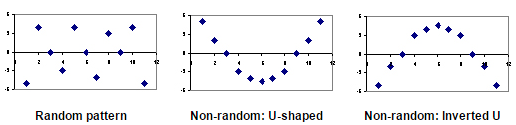
\includegraphics[width=120mm]{residual.png}
        \caption{Residual Plots}
        \label{fig:my_label}
\end{figure}
\subsection{Transformation}
\begin{objectives}
    \item Understand the purpose and reason of power transformation
    \item Know how to do power transformation
\end{objectives}
\vbox{}
After we do the Residual Plot analysis, we may find out the relationship between data set is nonlinear(it turns out the residual plot has a nonrandom pattern). Then it's sometimes possible for us to use the technique \Index{Power Transformation} to make the data linear for us to do linear regression.
\begin{Center}
    \textbf{Methods of Transformation}
\end{Center}
Transformation is using a simple function of a variable to rap lace the variable itself so that the scatter plot of the transformed data would appear to be linear. \\
\begin{examplebox}{Transformation}
    When we are unable to find a linear relationship between x and y, we instead try to find a linear regression between \(x^2\) and y. We can still predict y from x even though themselves are not linear related.
\end{examplebox}
\vbox{}
\begin{Center}
    \textbf{Most Common Ways of Transformation}
\end{Center}
\begin{figure}[H]
    \centering
        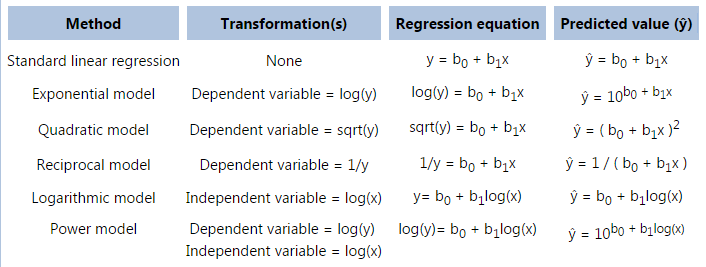
\includegraphics[width=150mm]{transformation.png}
        \caption{Transformation Methods}
        \label{fig:my_label}
\end{figure}
\begin{Center}
    \textbf{Some Important Notes}
\end{Center}
\begin{itemize}
    \item You can transform X or y or both of them.
    \item The residual plot of the transformed regression should has no pattern.
    \item The \(R^2\) and r of the transformed regression should be higher than the original one.
\end{itemize}
\subsection{Inferential of a Regression}
\begin{objectives}
    \item Know how to estimate variance of slope
    \item Understand confidence interval of slope
    \item Know how to test hypothesis with slope
\end{objectives}
\vbox{}
The \(b_1\) we get from all the data we have is actually just a point estimator of the true slope \Index{\(\beta_1\)}. And we can do all kinds of inferential methods just like we do with mean and proportions with the slope and the constant.
\begin{align}
    E(b_1)=\beta_1\\
    E(b_0)=\beta_0    
\end{align}

\begin{Center}
    \textbf{Assumptions}
\end{Center}
Before doing the inferences, we have to make some assumptions. \textcolor{red}{If the assumptions are satisfied, then we can continue with the inferential methods.}
\begin{enumerate}
    \item The errors are independent of each other.
    \item The errors follow a Normal Distribution.
    \item The variance of the errors is constant for all values of x.
\end{enumerate}
\vspace{3ex}
\begin{Center}
    \Index{Variance}
\end{Center}
When the above assumptions are true, then we can know that:
\begin{itemize}
    \item \(b_1\) has a Normal Distribution.
    \item \(\mu_{b_1}=\beta_1\)
\end{itemize}
Also we can get the \textbf{Variance of Coefficients}:
\begin{equation}
    \sigma_{b_1}=\frac{\sigma_e}{\sqrt{S_{xx}}}
\end{equation}
\begin{equation}
    \sigma_{b_0}=\frac{\sum{x_i}}{\sqrt{nS_{xx}}}\sigma_e
\end{equation}
\newpage
\begin{Center}
    \textbf{Confidence Interval}
\end{Center}
Doing confidence interval is just like all confidence interval we have learnt before.
\begin{equation}
    \beta_0\in (b_0\pm t_{c.l.}\sigma_{b_0})
\end{equation}
\begin{equation}
    \beta_1\in (b_1\pm t_{c.l.}\sigma_{b_1})
\end{equation}
However, \(\sigma^2e\) is unknown, we have to estimate it through:
\begin{equation}
    S^2_e=\frac{SSR}{n-2}
\end{equation}
\vspace{3ex}
\begin{Center}
    \textbf{Hypothesis Test}
\end{Center}
Testing the Slope is just like all hypothesis we have done before using a \textcolor{red}{t test}.\\
Normally, we would test if the there is a correlation between x and y; so our hypothesis would be:
\begin{itemize}
    \item \(H_0: \beta_1=0\)
    \item \(H_1: \beta_1\neq0\)
\end{itemize}
This test can ensure us that if we can reject the null hypothesis then we can use x t predict y. \\
The test statistic t would be:
\begin{equation}
    t=\frac{b_1-0}{s_b}
\end{equation}
In fact 0 can be changed to any value we want to test.\\
With the t we have, we can use calculator to get the p-value with a \textcolor{red}{df=n-2}.\\
Then we can make a conclusion using p-value and \(\alpha\) if there is one.
